\documentclass{beamer}

\usepackage{amsmath}
\usepackage{tikz}
\usepackage{ifthen}
\usepackage{hyperref}

\title{Zero-Knowledge Proofs}
\subtitle{Part 1: Knowing More Than Zero}
\author{Isaac Carruthers}

\tikzset{
    pics/my hat graph/.style n args={6}{
        code={
            \node[draw,fill=#1] at (0,0) (a) {A};
            \node[draw,fill=#2] at (0,1) (b) {B};
            \node[draw,fill=#3] at (1,0.5) (c) {C};
            \node[draw,fill=#4] at (2,0) (d) {D};
            \node[draw,fill=#5] at (2,1) (e) {E};
            \node[draw,fill=#6] at (3,1) (f) {F};
            \draw[] (a) -- (b);
            \draw[] (a) -- (c);
            \draw[] (c) -- (b);
            \draw[] (c) -- (e);
            \draw[] (c) -- (d);
            \draw[] (f) -- (e);
        }
    }
}

\begin{document}

\frame{\titlepage}

\frame{\frametitle{What do we Want?}
\centering
\begin{itemize}
	\item Peggy has some information, and he needs to prove some statement about it to Victor.
	\item Victor needs to verify that Peggy's statement is true.
	\item Peggy does not trust Victor, and does not want to show her anything beyond
	the fact that his statement is true.
\end{itemize}
}

\frame{\frametitle{What Guarantees do we Need?}
\centering
\begin{itemize}
	\item {\bf Completeness:} If the statement is true, then Victor should
	always be convinced that it is true.
	\item {\bf Soundness:} If the statement is false, there should be no way for Peggy
	to convince Victor.
	\item {\bf Zero-knowledge:} If the statement is true, Victor learns nothing other
	than the fact that the statement is true. Another way to frame this is that Victor
	already knows exactly what her interaction with Peggy will look like if the statement
	is true.
\end{itemize}
}

\frame{\frametitle{A Simple Example}
\centering
\begin{itemize}
	\item Peggy is not colorblind and claims two balls are different colors,
	but doesn't want to say what color they are.
	\item Victor is colorblind, and wants to be sure if Peggy is telling the truth.
	\item How do we work this out?
\end{itemize}
}

\frame{\frametitle{A Simple Example}
\centering
\begin{itemize}
	\item Victor puts both balls behind his back, then holds out just the one in his right hand.
	\item He then repeatedly brings the ball back behind his back, chooses
	whether to secretly switch them, and then holds out the one in his right
	hand again.
	\item Peggy tells him whether or not he switched them.
\end{itemize}
}

\frame{\frametitle{A Simple Example}
\centering
Does this meet our criteria?
\begin{itemize}
	\item {\bf Completeness:} If Victor keeps this up long enough, the chance that Peggy
	could just be guessing correctly will vanish, and Victor will be convinced.
	\pause
	\item {\bf Soundness:} By the same token, Peggy can't correctly say whether the balls
	were switched unless they are actually different colors.
	\pause
	\item {\bf Zero-knowledge:} Victor knows nothing at all except that the balls are
	different colors. Victor, knowing whether he has switched the balls or not, knows
	exactly how Peggy will respond each round if she's telling the truth, so he learns
	nothing new by hearing her response.
	\pause
	\item {\bf Yay!} It works.
\end{itemize}
}

\frame{\frametitle{A Bigger Problem}
\begin{itemize}
	\item I have a big graph, but Google has a big computer.
	\item I want to pay Google to figure out a 3-coloring for my graph.
	\item BUT! We live in a cryptopia, where monetary transactions are instant
	and irrevocable, and trust counts for nothing.
	\item How do I know Google has solved my problem before I give them my money?
\end{itemize}
\vspace{12pt}
\centering
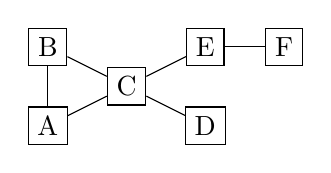
\begin{tikzpicture}
    \draw pic {my hat graph={white}{white}{white}{white}{white}{white}};
\end{tikzpicture}
}

\frame{\frametitle{Beginnings of a Solution}
\begin{enumerate}
	\item I agree on 3 colors with Google.
	\item Google rents out a warehouse, and lays out a colored version of my graph.
	\item Google covers every node with a hat, so I can't see the colors.
	\item I enter the warehouse, and pick an edge.
	\item Google uncovers both nodes connected to the edge, and I check that:
	\begin{enumerate}
		\item both nodes are one of the three agreed-upon colors,
		\item and they are different colors.
	\end{enumerate}
\end{enumerate}
}

\frame{\frametitle{Beginnings of a Solution}
\centering
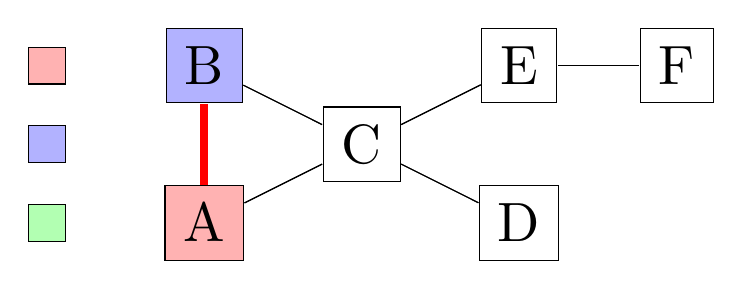
\begin{tikzpicture}[scale=2, every node/.style={scale=2}]
	\node[draw,fill=red!30] at (-1, 1) (x) {};
	\node[draw,fill=blue!30] at (-1, 0.5) (y) {};
	\node[draw,fill=green!30] at (-1, 0) (z) {};
    \draw pic {my hat graph={white}{white}{white}{white}{white}{white}};
	\pause
	\draw[line width=1mm,red] (a) -- (b);
	\pause
    \draw pic {my hat graph={red!30}{blue!30}{white}{white}{white}{white}};
	\draw[line width=1mm,red] (a) -- (b);
\end{tikzpicture}
}

\frame{\frametitle{So What?}
\centering
\begin{itemize}
	\item We've learned that Google laid out a graph where those two nodes
	were not the same color.
	\item We haven't learned anything else about the solution (we've seen nothing more
	than exactly what we were expecting to see; we could have simulated this result ourselves).
\end{itemize}
}

\frame{\frametitle{What About the Rest of the Graph}
\centering
\begin{itemize}
	\item Other parts of the graph could still be miscolored... How do we deal with that?
	\pause
	\item Do it over again! \pause (A lot!)
	\pause
\end{itemize}
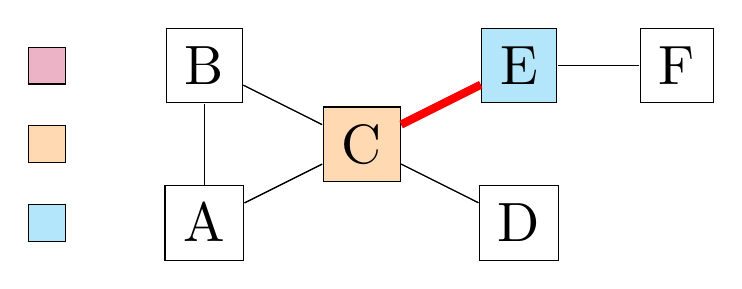
\begin{tikzpicture}[scale=2, every node/.style={scale=2}]
	\node[draw,fill=purple!30] at (-1, 1) (x) {};
	\node[draw,fill=orange!30] at (-1, 0.5) (y) {};
	\node[draw,fill=cyan!30] at (-1, 0) (z) {};
    \draw pic {my hat graph={white}{white}{white}{white}{white}{white}};
	\pause
	\draw[line width=1mm,red] (c) -- (e);
	\pause
    \draw pic {my hat graph={white}{white}{orange!30}{white}{cyan!30}{white}};
	\draw[line width=1mm,red] (c) -- (e);
\end{tikzpicture}
}

\frame{\frametitle{An Interesting Aside}
\centering
\begin{itemize}
	\item Now convinced, we take a recording of our hat procedure to our budgeting department
	to convince them to write a cheque to Google.
	\item Assuming they don't already trust us, should they believe that the solution exists
	based on the video?
	\pause
	\item No!
	\item It's the {\em interaction itself}, the challenge and response protocol, that convinced
	us Google had a solution.
	\item This is a direct consequence of the zero-knowledgeness! We knew exactly what to expect
	if they did have the solution, so we easily could have faked that outcome.
\end{itemize}
}

\frame{\frametitle{How do you Implement Hats in a Computer?}
\centering
\begin{itemize}
	\item The hats allowed Google to {\em commit} to a certain value for the colors of the graph.
	\item They also allowed Google to hide the values until they chose to reveal them.
	\item How can we do this with computers?
	\pause
	\item Google can just generate some random $k_i$, then give us $\mbox{Hash}(k_i || c_i)$
	for each node $i$ in the graph.
	\item When we challenge an edge, Google just gives us $k_i$ and $c_i$ for each of the two
	nodes on the edge, and we verify that the hashes match!
\end{itemize}
}

\frame{\frametitle{Weird Places we can Take This}
\centering
\begin{itemize}
	\item What if we made the committments... HOMOMORPHIC?!?
	\pause
	\item What if we made them homomorphic... ON THE BLOCKCHAIN?!?!?
\end{itemize}
}

\frame{\frametitle{Sources}
\centering
\begin{itemize}
	\item Thanks to \url{blog.cryptographyengineering.com} for the hats example.
	\item Thanks to \texttt{TikZ} for making diagrams fun, and also for teaching me
	another recursive acronym.
\end{itemize}
}

\end{document}
